% !TeX root = ../../Book3.tex
\section{伪双曲距离}
\label{b3:sec:0602}

Schwarz 引理比较的是点与原点的距离。若要比较任意两点，第一步应当把其中一点送到原点，而不是在原有坐标中直接平移：平移一般不保持单位圆盘。上一节的自同构
\[
 \phi_w(z)=\frac{z-w}{1-\overline w z}
\]
正好完成所需的换坐标。它在 \(z=w\) 时为零，且把整个单位圆盘仍映到自身。因此 \(|\phi_w(z)|\) 是从 \(w\) 出发测量 \(z\) 的自然候选量。本节先证明它确实给出一个不依赖圆盘坐标选择的距离，再计算它的球；下一节才引入一般全纯映射的压缩性质。

\subsection{伪双曲距离}
\label{b3:subsec:060201}

\Needspace{6\baselineskip}
\begin{definition}\label{b3:def:06-pseudohyperbolic}
对 \(z,w\in\mathbb D\)，定义\term[weishuangqu-juli]{伪双曲距离}[pseudohyperbolic distance]
\[
 \delta(z,w)\coloneqq\left|\frac{z-w}{1-\overline w z}\right|.
\]
\end{definition}
\symidx{\(\delta(z,w)\)：圆盘伪双曲距离}
因为 \(|\overline w z|<1\)，分母不为零。为检查其数值范围，展开得
\[
 |1-\overline w z|^2-|z-w|^2
 =(1-|z|^2)(1-|w|^2)>0,
\]
从而
\[
 1-\delta(z,w)^2
 =\frac{(1-|z|^2)(1-|w|^2)}{|1-\overline w z|^2}>0.
\]
于是 \(0\le\delta(z,w)<1\)，且只有 \(z=w\) 时等于零。交换 \(z,w\) 后分母变为原分母的共轭，分子的模不变，所以 \(\delta\) 对称。名称中的“伪”不表示不满足三角不等式；下面将证明它是一个真正的度量。它与第13章的 Poincaré 距离有关系
\[
 \mathrm d_{\mathbb D}(z,w)=2\operatorname{arctanh}\delta(z,w),
\]
其中右端的变换把有界区间 \([0,1)\) 变成 \([0,\infty)\)。

\ProseParagraphBreak

当 \(w=0\) 时 \(\delta(z,0)=|z|\)。当两点同时靠近边界时，情况不同。令 \(0<r<1\)，取
\[
 z=r,\quad w=\frac{1+r}{2}.
\]
欧氏位移为 \((1-r)/2\)，而
\[
 \delta\left(r,\frac{1+r}{2}\right)
 =\frac{(1-r)/2}{1-r(1+r)/2}
 =\frac1{2+r}\longrightarrow\frac13
 \quad(r\uparrow1).
\]
分子与分母同时变小，不能只根据分子趋于零就断言距离趋于零。两个点相对边界的距离处在相同量级，换到随观察点移动的圆盘坐标后，它们仍然保持可见的间隔。

在远离边界的固定紧盘上，两种距离则可以统一比较。若 \(|z|,|w|\le r<1\)，由
\[
 1-r^2\le |1-\overline w z|\le1+r^2
\]
得到
\[
 \frac{|z-w|}{1+r^2}\le\delta(z,w)
 \le\frac{|z-w|}{1-r^2}.
\]
因此对取值均在这个紧盘内的点列或函数族，收敛、Cauchy 性和一致收敛可以在两种距离之间换算。特别地，\(\delta\) 与欧氏距离在 \(\mathbb D\) 上给出相同的拓扑。具体说，若 \(z_n\to z\in\mathbb D\) 为欧氏收敛，则序列尾部和 \(z\) 落在某个固定紧盘内，以上估计给 \(\delta(z_n,z)\to0\)；反向由全域成立的
\[
 |z-w|=\delta(z,w)\cdot|1-\overline w z|
 \le2\delta(z,w)
\]
即可得到欧氏收敛。这一结论只比较圆盘内的极限，不能把落在单位圆周上的欧氏极限当作该度量空间中的点。

\ProseParagraphBreak

固定 \(a\in\mathbb D\)，还有局部尺度公式
\[
 \lim_{\substack{z\to a\\z\ne a}}
 \frac{\delta(z,a)}{|z-a|}
 =\frac1{1-|a|^2}.
\]
其依据只是分母的连续性。它说明同样大小的微小欧氏位移，在边界附近对应更大的伪双曲位移。这里先得到局部比值；沿曲线积分所形成的几何将在第13章另行建立。

\subsection{圆盘自同构不变性}
\label{b3:subsec:060202}

\Needspace{6\baselineskip}
\begin{proposition}\label{b3:prop:06-mobius-invariance}
单位圆盘自同构 \(T:\mathbb D\to\mathbb D\) 对所有 \(z,w\in\mathbb D\) 满足 \(\delta(Tz,Tw)=\delta(z,w)\)。此外，对任意 \(z,w,a\in\mathbb D\)，
\[
 \delta(z,w)\le\frac{\delta(z,a)+\delta(a,w)}{1+\delta(z,a)\cdot\delta(a,w)}
 \le\delta(z,a)+\delta(a,w).
\]
\end{proposition}
\begin{proof}
旋转保持分式的模。对 \(\phi_a(z)=(z-a)/(1-\overline a z)\)，分别通分，得到
\[
 \phi_a(z)-\phi_a(w)
 =\frac{(1-|a|^2)(z-w)}{(1-\overline a z)(1-\overline a w)},
\]
\[
 1-\overline{\phi_a(w)}\phi_a(z)
 =\frac{(1-|a|^2)(1-\overline w z)}
 {(1-a\overline w)(1-\overline a z)}.
\]
因 \(a,z,w\in\mathbb D\)，所写各分母及 \(1-\overline w z\) 都不为零；\(1-|a|^2>0\)，故两式可相除并约去公共因子，得到
\[
 \frac{\phi_a(z)-\phi_a(w)}
 {1-\overline{\phi_a(w)}\phi_a(z)}
 =\frac{z-w}{1-\overline w z}
   \frac{1-a\overline w}{1-\overline a w}.
\]
最后一个因子的分子与分母互为共轭，模为1。取绝对值即得 \(\delta(\phi_a(z),\phi_a(w))=\delta(z,w)\)。圆盘自同构都是旋转与某个 \(\phi_a\) 的复合，所以一般的 \(T\) 也保持 \(\delta\)。

证明三角不等式时，用 \(\phi_a\) 将中间点移到0，令
\[
 p=\phi_a(z),\quad q=\phi_a(w),\quad
 r=|p|=\delta(z,a),\quad s=|q|=\delta(a,w).
\]
若 \(r=0\) 或 \(s=0\)，所需分式不等式直接取等。以下设 \(r,s>0\)，记
\[
 t=\frac{\operatorname{Re}(p\overline q)}{rs}\in[-1,1].
\]
由不变性及距离公式，
\[
 \delta(p,q)^2=\frac{r^2+s^2-2rst}{1+r^2s^2-2rst}.
\]
将右端看成 \(t\) 的函数 \(F(t)\)，其导数为
\[
 F'(t)=
 -\frac{2rs(1-r^2)(1-s^2)}
 {(1+r^2s^2-2rst)^2}<0.
\]
故最大值在 \(t=-1\) 达到，此时分子为 \((r+s)^2\)，分母为 \((1+rs)^2\)。开平方即得第一重不等式。又因 \(1+rs\ge1\)，得到通常三角不等式，结合前面的对称性和正定性可知 \(\delta\) 是度量。
\end{proof}
选择把中间点送到0，是为了把三个任意位置的点化成两个模和一个夹角。

当 \(z\ne a\)、\(w\ne a\) 时，导数的严格负号还给出了第一重不等式的精确等号条件：
\[
 \frac{\phi_a(z)}{|\phi_a(z)|}
 =-\frac{\phi_a(w)}{|\phi_a(w)|}.
\]
也就是说，把 \(a\) 送到0后，另两点落在同一直径的两侧。原坐标中的相应曲线是该直径的自同构逆像；若它是直线，就是过原点的直径，否则是与单位圆正交的圆弧。这里可以用分式线性变换把广义圆映为广义圆、并在单位圆附近保角来识别曲线的形状。此时尚未用长度刻画这些曲线；第13章才证明它们是双曲测地线。

\ProseParagraphBreak
通常的加法三角不等式在 \(z\ne a\)、\(w\ne a\) 时总是严格的，因为 \((r+s)/(1+rs)<r+s\)。例如三点 \(-s,0,r\) 位于实轴上，虽然第一重分式不等式取等，却有
\[
 \delta(-s,r)=\frac{r+s}{1+rs}<r+s
 =\delta(-s,0)+\delta(0,r).
\]
因此不能直接把 \(\delta\) 当作沿这条直线可加的长度。反双曲正切的加法公式恰好处理这个差异：
\[
 \operatorname{arctanh}\frac{r+s}{1+rs}
 =\operatorname{arctanh}r+\operatorname{arctanh}s.
\]
由于 \(\operatorname{arctanh}\) 递增，分式三角不等式也立即保证 \(2\operatorname{arctanh}\delta\) 满足通常三角不等式。它与路径长度的一致性仍需要后续证明。

\subsection{几何解释}
\label{b3:subsec:060203}

距离已经确定后，可以具体问：从 \(a\) 看去不超过某个固定尺度的点，在原来的欧氏坐标中形成什么集合？由定义，该集合是 \(\phi_a^{-1}\) 对一个同心小圆盘的像。下面直接计算其圆心与半径，以便区分两套坐标中的“中心”。

\Needspace{6\baselineskip}
\begin{proposition}\label{b3:prop:06-pseudohyperbolic-ball}
设 \(a\in\mathbb D\)、\(0<r<1\)。开伪双曲球
\[
 B_\delta(a,r)\coloneqq\{z\in\mathbb D:\delta(z,a)<r\}
\]
等于欧氏圆盘 \(D(c,R)\)，其中
\[
 c=\frac{(1-r^2)a}{1-r^2|a|^2},\quad
 R=\frac{r(1-|a|^2)}{1-r^2|a|^2}.
\]
相应的闭球为 \(\overline{D(c,R)}\)，并且
\[
 |c|+R=\frac{|a|+r}{1+r|a|}<1.
\]
特别地，每个半径小于1的闭伪双曲球都是 \(\mathbb D\) 内的欧氏紧集。
\end{proposition}
\begin{proof}
将 \(\delta(z,a)<r\) 等价地写成
\(|z-a|^2<r^2|1-\overline a z|^2\)，展开两边得
\[
 (1-r^2|a|^2)|z|^2
 -2(1-r^2)\operatorname{Re}(\overline a z)+|a|^2-r^2<0.
\]
首项系数 \(A=1-r^2|a|^2\) 为正，除以 \(A\) 后配方。中心为 \(c=(1-r^2)a/A\)，半径的平方为
\[
 |c|^2-\frac{|a|^2-r^2}{A}
 =\frac{(1-r^2)^2|a|^2-(|a|^2-r^2)(1-r^2|a|^2)}{A^2}
 =\frac{r^2(1-|a|^2)^2}{A^2}.
\]
这给出所述 \(c,R\)。还须检查算出的整个欧氏盘确实位于原定义域中。令 \(s=|a|<1\)，则
\[
 |c|+R
 =\frac{(1-r^2)s+r(1-s^2)}{1-r^2s^2}
 =\frac{s+r}{1+sr}<1,
\]
最后一个严格不等式等价于 \((1-s)(1-r)>0\)。因而该圆盘连同边界都包含在 \(\mathbb D\) 中。把推导中的严格不等号换成非严格不等号，便得到闭球公式；其欧氏闭性、有界性给出紧性。
\end{proof}

若 \(a\ne0\)，则系数 \((1-r^2)/(1-r^2|a|^2)\) 在0与1之间，所以欧氏圆心 \(c\) 位于原点与内在球心 \(a\) 之间。它们不是同一个点。距离球在 \(a\) 两侧的欧氏宽度不同，是因为朝向单位圆的一侧具有较大的局部度量尺度。

\begin{figure}[htbp]
\centering
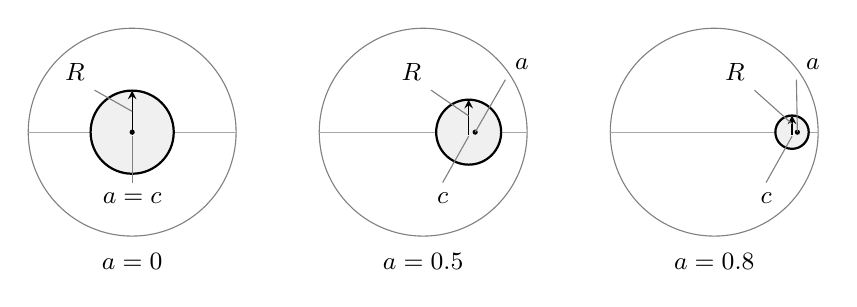
\begin{tikzpicture}[>=stealth,font=\small,scale=1.32]
 \foreach \shift/\a/\c/\rad in {0/0/0/0.4,2.8/0.5/0.4375/0.3125,5.6/0.8/0.74866/0.16043}{
  \begin{scope}[xshift=\shift cm]
   \draw[gray] (0,0) circle (1);
   \draw[gray!70] (-1,0)--(1,0);
   \draw[thick,fill=gray!12] (\c,0) circle (\rad);
   \draw[->] (\c,0)--(\c,\rad);
   \node at (\c-0.55,0.58) (radiuslabel) {\(R\)};
   \draw[gray] (radiuslabel.south east)--(\c,0.5*\rad);
   \draw (\c,-0.025)--(\c,0.025);
   \fill (\a,0) circle (0.025);
   \ifdim\a pt=0pt
    \node at (\c,-0.63) (centerlabel) {\(a=c\)};
    \draw[gray] (centerlabel.north)--(\c,-0.04);
   \else
    \node at (\c-0.25,-0.63) (centerlabel) {\(c\)};
    \draw[gray] (centerlabel.north)--(\c,-0.04);
    \node at (0.95,0.65) (pointlabel) {\(a\)};
    \draw[gray] (pointlabel.south west)--(\a,0);
   \fi
   \node[below] at (0,-1.07) {\(a=\a\)};
  \end{scope}
 }
\end{tikzpicture}
\caption[固定伪双曲半径的球]{三个圆盘都满足 \(\delta(z,a)<2/5\)，按同一欧氏尺度绘制。实心点是内在球心 \(a\)，短标记是欧氏圆心 \(c\)；第一图二者重合。由左向右，内在半径不变，欧氏半径 \(R\) 缩小，圆心差也须由公式而不是目测判断。}
\label{b3:fig:06-pseudohyperbolic-balls}
\end{figure}

\cref{b3:fig:06-pseudohyperbolic-balls}固定的是 \(r=2/5\)，而不是欧氏半径 \(R\)。在每幅图中用 \(\phi_a\) 把实心点送到原点后，小圆盘都变成同一个 \(|w|<2/5\)。

\ProseParagraphBreak

球公式给出它离单位圆的最小欧氏间隙：
\[
 1-|c|-R
 =\frac{(1-|a|)(1-r)}{1+r|a|}.
\]
对固定的 \(a,r\)，这个数为正；当中心趋向边界或半径趋向1时，它可以趋于零。因而每一个这样的闭球都是紧的，并不意味着所有闭球可被某一个共同的圆盘内紧集包住。

\ProseParagraphBreak

由距离不变性，每个圆盘自同构 \(T\) 满足
\[
 T(B_\delta(a,r))=B_\delta(T(a),r).
\]
这里等号的一个包含由 \(T\) 的不变性得到，另一个包含对 \(T^{-1}\) 使用同一性质得到。因此换坐标保留的是伪双曲半径 \(r\)，图中的欧氏半径 \(R\) 可以改变。这也解释了为什么一个自同构能在某点放大欧氏长度，同时仍保持所有伪双曲距离。

给定中心 \(a\) 的伪双曲球半径 \(r\) 增大时，欧氏中心从 \(a\) 沿径向移向0，欧氏半径增大。这不是一个固定圆心的同心圆族，却同样构成邻域基。若 \(a\) 为正实数，球与实轴的交点可直接由 \(|(x-a)/(1-ax)|=r\) 解出：
\[
 x_- =\frac{a-r}{1-ar},\quad x_+=\frac{a+r}{1+ar}.
\]
它们的平均数与半差恰为上面的 \(c,R\)，提供配方公式的另一检验。实轴上的这两个端点以后也是双曲距离计算中最简单的坐标。

\ProseParagraphBreak
这两个端点还可以量化边界附近的形状。若 \(a\in(0,1)\)，则
\[
 a-x_-=\frac{r(1-a^2)}{1-ar},\quad
 x_+-a=\frac{r(1-a^2)}{1+ar}.
\]
朝向右边界的宽度较小。当 \(a\uparrow1\) 而 \(r\) 固定时，
\[
 \frac{R}{1-a}\longrightarrow\frac{2r}{1-r^2},\quad
 \frac{1-x_+}{1-a}\longrightarrow\frac{1-r}{1+r},\quad
 \frac{1-x_-}{1-a}\longrightarrow\frac{1+r}{1-r}.
\]
所以整个小圆盘向边界收缩的尺度与 \(1-a\) 相当，但在以 \(a\) 为原点的圆盘坐标中，它始终是同一个半径 \(r\) 的盘。相反，固定 \(a\) 而令 \(r\uparrow1\) 时，\(c\to0\)、\(R\to1\)，这些球递增穷尽 \(\mathbb D\)。两种极限固定的参数不同，几何结果也不同。

\ProseParagraphBreak

现在可以证明一个容易与“距离有界”混淆的事实。

\Needspace{6\baselineskip}
\begin{proposition}\label{b3:prop:06-pseudohyperbolic-complete}
单位圆盘配备伪双曲距离 \(\delta\) 后是完备度量空间：每个 \(\delta\)-Cauchy 列都在 \(\mathbb D\) 中关于 \(\delta\) 收敛。
\end{proposition}
\begin{proof}
设 \((z_n)\) 是 \(\delta\)-Cauchy 列。取 \(N\)，使 \(m,n\ge N\) 时 \(\delta(z_m,z_n)<1/2\)。固定 \(a=z_N\)，序列尾部便包含在闭球 \(\overline B_\delta(a,1/2)\) 中。由 \cref{b3:prop:06-pseudohyperbolic-ball}，存在 \(\rho<1\)，使这个闭球包含于 \(\{|z|\le\rho\}\)。

由 \(|z_m-z_n|\le2\delta(z_m,z_n)\)，该序列是欧氏 Cauchy 列，故收敛到某个 \(z\in\mathbb C\)。尾部位于上述欧氏闭球，因而极限仍在其中，特别地 \(|z|\le\rho<1\)。再用固定紧盘上的比较式，
\[
 \delta(z_n,z)\le\frac{|z_n-z|}{1-\rho^2}\longrightarrow0
 \quad(n\ge N).
\]
这就是所需的圆盘内极限。
\end{proof}

完备性要求 Cauchy 列具有空间内极限，并不要求距离函数无界。例如取 \(z_n=1-1/n\)，\(n\ge2\)，则欧氏意义下相邻项越来越接近边界，但
\[
 \delta(z_n,z_{2n})=\frac{n}{3n-1}\longrightarrow\frac13.
\]
所以它甚至不是 \(\delta\)-Cauchy 列。这里不能只检查相邻两项的距离；Cauchy 条件要求所有充分晚的两项同时接近。闭球公式保证真正的 \(\delta\)-Cauchy 列最终留在圆盘内部的某个紧集，这正是边界点不会作为遗漏极限出现的原因。

下一节将证明任意圆盘全纯自映射都不增加 \(\delta\)。届时，不变性描述的自同构将成为压缩估计的等号情形，而本节的局部尺度公式将把两点估计转成导数估计。
